\chapter{Optical Quality Metrics: MTF, OTF, and the Strehl Ratio}
\label{ch:mtf_strehl}

Stage 3 (\texttt{stage3\_human\_vision/}) adds a battery of standard optical-quality
metrics on top of Stage 2's retinal PSF, as the bridge into the human-vision models of
Chapters~\ref{ch:csf}--\ref{ch:stage4}.

\section{MTF and OTF from the PSF}

The complex optical transfer function is the normalized Fourier transform of the PSF,
radially averaged into 1-D:
\begin{equation}
\text{OTF}(f) = \frac{\big\langle \mathcal{F}\{I(x,y)\}\big\rangle_{|f_x,f_y|=f}}
{\mathcal{F}\{I\}(0,0)}, \qquad \text{MTF}(f)=|\text{OTF}(f)|.
\end{equation}
Retina-plane spatial frequency (cycles/\textmu m) converts to the clinically standard
cycles/degree of visual angle via the eye's own posterior nodal distance $v_r$
(small-angle approximation): $1^\circ$ subtends $v_r\tan(1^\circ)\approx v_r\,(\pi/180)$
at the retina. MTF50 and MTF10 (the frequencies at which MTF drops to $50\%$ and
$10\%$ of its DC value) are reported as two candidate resolution-limit criteria.

\section{Strehl ratio}

\begin{equation}
S = \frac{I_{peak,actual}/P_{actual}}{I_{peak,DL}/P_{DL}}
\end{equation}
comparing peak PSF intensity (each normalized by its own total power first) against a
diffraction-limited reference --- \textbf{this project's fixed convention: the same
system's own $M=0$ (zero-defocus, emmetropic) PSF at the same $(a_{hole}, \lambda,
d_{gap})$}, not an idealized Airy disk.

\subsection*{Finding: the Strehl ratio is not well-posed in this near-field regime}

A direct numerical scan of peak retinal intensity vs.\ propagation distance $v_r$, at
fixed $a_{hole}=750\um$, found peak intensity is \textbf{not} single-peaked in $v_r$ ---
it oscillates, the same near-field Fresnel behavior as Stage 1's own on-axis
oscillation formula (Chapter~\ref{ch:stage1}). Concretely, that scan found a peak of
$1239$ (a.u.) at $v_r=29\mm$, against only $\approx76$--$77$ at $v_r=23$--$25\mm$ ---
precisely where $M=4$--$5\,$D actually places the retina. \textbf{This means $M=0$ is
demonstrably not always the true best-focus condition}, so Strehl computed against the
$M=0$ reference \emph{can legitimately exceed $1.0$} for some $(a_{hole}, M)$
combinations --- confirmed directly in this report's own sweeps (Figure~\ref{fig:strehl-heatmap}),
reaching values as high as $\approx3.7$ at $M=8\,$D. This is not a code bug; it is a
property of operating in the Fresnel near-field regime ($N_F\gtrsim1$), where the
classical Strehl ratio --- built for mildly-aberrated, near-diffraction-limited systems
with one well-defined focus --- is not a well-posed metric. Every chapter downstream
that reports Strehl explicitly carries this caveat rather than treating
Strehl-exceeds-unity points as errors.

\begin{figure}[htbp]
\centering
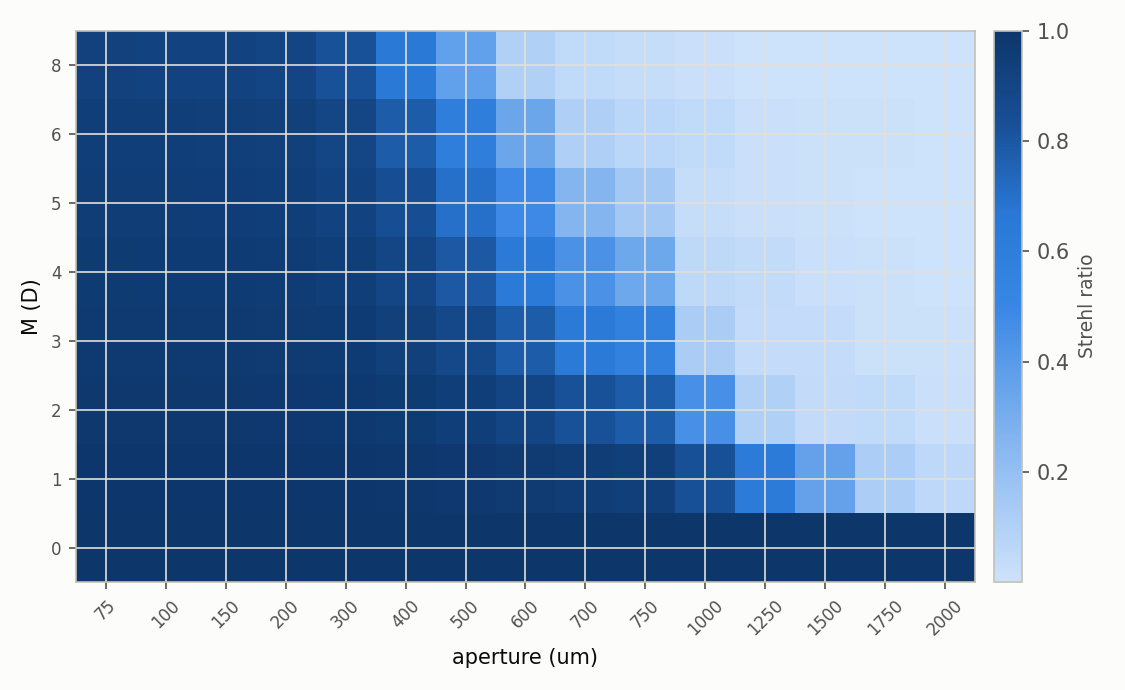
\includegraphics[width=0.85\textwidth]{figures/fig_strehl_heatmap.png}
\caption{Strehl ratio across the full aperture $\times$ myopia grid --- note values exceeding 1.0 at high $M$, a genuine near-field effect, not an artifact.}
\label{fig:strehl-heatmap}
\end{figure}

\section{A related, similarly unstable metric: FWHM}

FWHM (Section~\ref{sec:effective-radius}) is subject to the same ring-hopping
instability documented at the corneal plane in Stage 1 --- and confirmed \emph{worse}
at the retina plane, where the profile's peak/crossing point can hop between Fresnel
rings for adjacent aperture values only a few microns apart. Every FWHM value reported
anywhere in this project's sweeps carries its crossing mode and crossing count
alongside the radius, specifically so an unstable reading is visible rather than
silently trusted as a clean number. \textbf{Neither Strehl nor FWHM should be used as a
primary design metric in this regime without further work} --- $r_{EE}(P)$ and RMS
radius, which integrate over structure rather than reading one potentially-lucky peak
or crossing, are preferred throughout this report.

{\small
\begin{longtable}{rrrrrr}
\caption{Stage 3 optical-quality metrics at aperture=750um, all myopia levels.}\label{tab:mtf-strehl-full}\\
\toprule
M (D) & MTF50 (cpd) & MTF10 (cpd) & Strehl & Strehl>1 & RMS radius (um) \\
\midrule
\endfirsthead
\multicolumn{6}{c}{\tablename\ \thetable\ -- continued}\\
\toprule
M (D) & MTF50 (cpd) & MTF10 (cpd) & Strehl & Strehl>1 & RMS radius (um) \\
\midrule
\endhead
\bottomrule
\endfoot
0.000 & 12.840 & 25.597 & 1.000 & False & 82.924 \\
1.000 & 11.993 & 25.773 & 0.937 & False & 83.439 \\
2.000 & 9.548 & 25.558 & 0.778 & False & 84.222 \\
3.000 & 7.138 & 23.944 & 0.559 & False & 85.294 \\
4.000 & 5.510 & 12.892 & 0.333 & False & 86.675 \\
5.000 & 4.445 & 8.918 & 0.149 & False & 88.382 \\
6.000 & 3.712 & 6.941 & 0.071 & False & 90.433 \\
8.000 & 2.784 & 4.862 & 0.032 & False & 95.626 \\
\end{longtable}
}
